\chapter{Probleme, Komplexität und Berechnungsmodelle}
\section{Fünf Algorithmen zum Sortieren}
Betrachten wir beispielhaft ein Problem und verschiedene Algorithmen zu seiner Lösung. Anschließend können wir die Algorithmen miteinander vergleichen.

\subsection{Die Algorithmen\dots}
\begin{Prob}
\hspace{\parindent}Gegeben ist die Eingabe $S = a_1, \ldots, a_n$, mit $a_i \in \mathcal{U}$. Auf $\mathcal{U}$ ist eine totale Ordnung $\le$ definiert.
Gewünscht ist eine Permutation $\pi$ mit $a_{\pi(1)}~\le \ldots \le a_{\pi(n)}$. Dies kann nur erreicht werden, in dem ein Algorithmus die Eingabe umsortiert.
\end{Prob}

\begin{Alg}[Bogosort]\label{Bogosort}
\begin{enumerate}
\item Erzeuge systematisch alle Permutaionen $\pi$ von $\{a_1 \ldots a_n\}$.
\item Teste, ob die erzeugte Permutation $a_{\pi(1)} \le \ldots \le a_{\pi(n)}$ entspricht.
\item Ist die gewünschte Permutation gefunden, brich ab.
\end{enumerate}
\end{Alg}

\begin{Alg}[Sortieren durch Auswahl]\label{Sortieren-durch-Auswahl}
\begin{enumerate}
\item Durchlaufe die Eingabefolge und finde ihr Minimum.
\item Gebe das gefundene Minimum aus.
\item Wiederhole die ersten beiden Schritte mit der Restfolge, bis die ganze Folge abgearbeitet ist.
\end{enumerate}
\end{Alg}

\begin{Alg}[Mergesort]\label{Mergesort}
\begin{enumerate}
\item Falls die Folge nur aus einem Element besteht: gib dieses aus.
\item Sonst: Teile die Eingabefolge $S$ in zwei Teilfolgen $S_1 = a_1, \ldots a_{\frac{n}{2}}$ und $S_2 = a_{\frac{n}{2}} \ldots a_n$.
\item Sortiere $S_1$ und $S_2$ rekursiv.
\item Mische beide sortierten Teilfolgen zu einer sortierten Gesamtfolge, wobei die einzelnen Elemente von $S_1$ mit denen von $S_2$ verglichen werden.
\end{enumerate}
\end{Alg}

\begin{Alg}[Quicksort]\label{Quicksort}
\begin{enumerate}
\item Falls $|S| = 1$ gibt $S$ aus, sonst:
\item Wähle zufällig ein Element $a$ aus und teile $S$ in $S_1$ (Elemente $\le a$) und $S_2$ (Elemente $>a$).
\item Sortiere rekursiv $S_1$ und $S_2$
\item Gib aus $S_1$ (sortiert), a, $S_2$ (sortiert).
\end{enumerate}
\end{Alg}

Dieser Algorithmus wählt ein Element zufällig aus, die Rolle des Zufalls müssen wir noch genauer untersuchen.

\begin{Alg}\label{Alter-Mann}
\begin{enumerate}
\item Wähle zufällig zwei Elemente aus $S$ aus $a_i, a_j \in S$ mit $i < j$.
\item Für den Fall, dass sie in der falschen Reihenfolge sind, das heißt $a_i > a_j$, vertausche sie.
\item Wiederhole den Prozess $k(n)$-mal.
\end{enumerate}
\end{Alg}

\begin{Bem}[Monte-Carlo-Algorithmen]\label{Monte-Carlo}
\hspace{\parindent}Ist das ein richtiger Algorithmus? Es gibt eine Wahrscheinlichkeit, dass wir immer die beiden selben Elemente auswählen und die anderen Elemente unsortiert bleiben. Solche Algorithmen werden\textit{ Monte-Carlo-Algorithmus} genannt. Die Wahrscheinlichkeit von einem Monte-Carlo-Algorithmus ein falsches Ergebnis zu erhalten sollte nach oben hin beschränkt sein. Monte-Carlo-Algorithmen werden genutzt wenn die Wahrscheinlichkeit ein falsches Ergebnis zu bekommen gering, die Algorithmen jedoch effizienter sind, als vergleichbare deterministische Algorithmen. Für obigen Algorithmus ist offen ist, wie groß $k(n)$ sein muss, um mit einer akzeptablen Wahrscheinlichkeit ein richtiges Ergebnis zu erzielen.
\end{Bem}

\subsection{\dots und ihre Effizienz}
Welcher der vorgestellten Algorithmen ist "`der Beste"'? Ein einfaches Maß ist die Anzahl der Vergleiche als Funktion abhängig von der Länge $n$ der Eingabefolge. Je nach Eingabe hat ein Algorithmus natürlich unterschiedliche Laufzeiten. Daher sollte, wo es relevant ist, der \textit{günstigste} und der \textit{schlechteste Fall}, sowie die Laufzeit \textit{im Mittel} untersucht werden.

\begin{Lza}[Bogosort]
\hspace{\parindent}Im günstigsten Fall ist die erste Permutation die richtige. Hierzu brauchen wir $n-1$ Vergleiche. Im schlechtesten Fall ist die letzte Permutation die richtige. Es gibt $n!$ viele Permutationen, das heißt wir brauchen $n!(n-1)$ Vergleiche.
\begin{align*}
  n! & = 1 \cdot 2 \cdot \ldots \cdot n \le n^n \\
  n! & = 1 \cdot 2 \cdot \ldots \cdot \frac{n}{2} \cdot (\frac{n}{2} + 1) \cdot \ldots \cdot n \ge (\frac{n}{2})^\frac{n}{2}
\end{align*}
Im Mittel können wir von ungefähr $\frac{n!}{2}(n-1)$ Vergleichen ausgehen.
\end{Lza}

\begin{Lza}[Sortieren durch Auswahl]
\hspace{\parindent}Die Laufzeit ist ziemlich klar: in der ersten Iteration müssen n-1 Vergleiche durchgeführt werden, um das Minimum zu finden. In der zweiten Iteration werden dann noch n-2 Vergleiche gebraucht, um das Minimum der Restfolge zu bestimmen, usw. Die Anzahl der Vergleiche lässt sich also wie folgt ermitteln:
\begin{align*}
  \sum_{k=1}^{n-1 }k &= \frac{n(n-1)}{2}\\
                     &= \frac{1}{2}n^2 - \frac{1}{2} n\\
                     &= \Theta(n^2)
\end{align*}
\end{Lza}

\begin{Lza}[Mergesort]
\hspace{\parindent}$C(n)$ sei die maximale Anzahl der Vergleiche bei Eingabe der Länge $n$. Wir können $C(n)$ rekursiv angeben:
\begin{align*}
  C(1) &= 0\\
  C(n) &= 2 \cdot C(\frac{n}{2}) + (n-1)
\end{align*}

Dabei gehen wir davon aus, dass es sich bei $n$ um eine Zweierpotenz handelt. $2 \cdot C(\frac{n}{2})$ berechnet die Anzahl der Vergleiche für die beiden rekursiven Aufrufe und $(n-1)$ steht für die Anzahl der Vergleiche beim Mischen der beiden Teilfolgen im schlechtesten Fall (es sind abwechselnd Elemente aus beiden Teilfolgen zu wählen). Im besten Fall haben wir es mit $\frac{n}{2}$ Vergleichen zu tun (erst alle Elemente einer Teilfolge, dann die übrigen Elemente der anderen Teilfolge). Aus der rekursiven Form können wir jedoch die Laufzeit nicht ablesen. Wir suchen daher eine geschlossene Form, unter der Annahme, dass es sich bei $n$ um eine Zweierpotenz handelt, also $n=2^k$ mit $k \ge 1$.
\begin{align*}
  C(n) &= 2 \cdot C(\frac{n}{2}) + (n-1)\\
       &\le 2 \cdot C(\frac{n}{2}) + n\\
       &\le 4 \cdot C(\frac{n}{4}) + 2 \cdot n\\
       &\ldots\\
       &\le 2^k \cdot C(\frac{n}{2^k}) + k \cdot n \\
       &\le 2^{\log_2 n} \cdot C(1) + \log_2 n \cdot n\\
       &\le n \log_2 n
\end{align*}
\end{Lza}

\begin{Lza}[Quicksort]\label{QuicksortLza}
\hspace{\parindent}Betrachten wir zu nächsten die Laufzeit im schlechtesten Fall $C_s$, falls das ausgewählte Element $a$ das größte oder kleinstes Element der Folge ist. Zunächst gilt der triviale Fall  $C_s(1) = 0$. Des Weiteren lässt sich $C_s$ rekursiv bestimmt als $C_s(n)  = C_s(n-1) + n-1$. Hierbei berechnet $C_s(n-1)$ die Vergleiche des rekursiven Aufrufs und $n-1$ die Vergleichsoperationen mit dem kleinsten oder größtem Element. Auch hier wollen wir wieder eine geschlossene Formel finden:
\begin{align*}
  C_s(n) &= n-1 + n-2 + \ldots + 1\\
         &= \frac{n(n-1)}{2}
\end{align*}

Betrachten wir den allgemeinen Fall. Auch hier gibt es den trivialen Fall $C(1) = 0$ und den rekursiven Fall $C(n) = C(k-1) + C(n-k) + n-1$. $C(k-1)$ berechnet die Anzahl der Vergleiche für den rekursiven Aufruf von $S_1$ und $C(n-k)$ die Anzahl der Vergleiche für den rekursiven Aufruf von $S_2$. $n-1$ steht für die Vergleiche, die zur Aufteilung der beiden Teilfolgen erforderlich sind. Da $k$ abhängig vom Zufall ist, können wir die Rekursion leider nicht auflösen.

Wir können die Anzahl der Vergleiche jedoch als Zufallsvariable auffassen und ihren Erwartungswert bestimmen, also die mittlere Anzahl der Vergleiche. $k$ kann die Werte $1, \ldots, n$ annehmen, d.h. das ausgewählte Element ist das $k$-te Element ($k$-größte Element) der Folge. Die Wahrscheinlichkeit für jedes $k$ entspricht $\frac{1}{n}$. Die obige Rekursionsgleichung lässt sich nun neu aufstellen:

\begin{align*}
  C(1) &= 0\\
  C(n) &=  \frac{1}{n} \sum_{k=1}^{n} \left( C(k-1) + C(n-k)\right) + n-1
\end{align*}

$\sum_{k=1}^{n} C(k-1)$ summiert $C(k)$ für alle $0 \le k \le n-1$ auf. $\sum_{k=1}^{n} C(n-k)$ summiert $C(k)$ für alle $n-1 \ge k \ge 0$ auf. Da es auf die Reihenfolge nicht ankommt, können wir die Summe verkürzen. Es gilt:
\[\sum_{k=1}^{n} \left( C(k-1) + C(n-k)\right)  = 2 \cdot \sum_{k=0}^{n-1} C(k)\]
Nun können wir die Gleichung weiter entwickeln. Wir multiplizieren mit $n$ und ersetzen $n$ durch $n-1$.
\begin{align*}
  n \cdot C(n) &= 2 \cdot \sum_{k=0}^{n-1} C(k) + n(n-1)\\
  (n-1) \cdot C(n-1) &= 2 \cdot \sum_{k=0}^{n-2} C(k) + (n-1)(n-2)
\end{align*}
Wir ziehen die zweite Zeile von der ersten ab und stellen um:
\begin{align*}
n \cdot C(n) - (n-1) \cdot C(n-1) &= 2 \cdot C(n-1) + 2(n-1)\\
n \cdot C(n) &= 2 \cdot C(n-1) + 2(n-1) +(n-1) \cdot C(n-1)\\
n \cdot C(n) &= (n+1) \cdot C(n-1) + 2(n-1)\\
C(n) &= \frac{n+1}{n} \cdot C(n-1) + 2\frac{n-1}{n}
\end{align*}
Wandeln wir die Gleichung in eine Ungleichung, können wir sie vereinfachen ($2 \ge 2 \frac{n-1}{n}$).
\[ C(n) \le \frac{n+1}{n} \cdot C(n-1) + 2 \]
Wir ersetzen $n$ erneut durch $n-1$
\[ C(n-1) \le \frac{n}{n-1} \cdot C(n-2) + 2 \]
fügen dies in $C(n)$ ein und erweitern die letzte $2$ um $\frac{n+1}{n+1}$:
\begin{align*}
  C(n) &\le \frac{n+1}{n} \cdot \left( \frac{n}{n-1} \cdot C(n-2) + 2 \right) + 2 \frac{n+1}{n+1}\\
       &\le \frac{n+1}{n-1} \cdot C(n-2) + 2 \frac{n+1}{n} + 2 \frac{n+1}{n+1}
\end{align*}
Wenn wir diesen Vorgang wiederholen, bekommen wir:
\begin{align*}
  C(n) &\le \frac{n+1}{n-1} \cdot \left( \frac{n-1}{n-2} \cdot C(n-3) + 2 \right) + 2 \frac{n+1}{n} + 2 \frac{n+1}{n+1}\\
       &\le \frac{n+1}{n-2} \cdot C(n-3) + 2 \frac{n+1}{n-1} + 2 \frac{n+1}{n} + 2 \frac{n+1}{n+1}\\
\end{align*}
Nun erkennen wir, worauf das hinausläuft:
\[ C(n) \le \frac{n+1}{2} C(1) + 2(n+1) \left( \frac{1}{1} + \frac{1}{2} + \ldots + \frac{1}{n-1} + \frac{1}{n} + \frac{1}{n+1} \right) \]

$H_n = \sum_{k=1}^{n}\frac{1}{k}$ nennt man auch die $n$. Harmonische Zahl. Wir verzichten auf einen Beweis per Induktion und erkennen an, dass es sich oben um die $(n+1)$-te Harmonische Zahl handelt. Wir wollen die Harmonische Zahl abschätzen.

\begin{figure}[hbt]
  \centering
  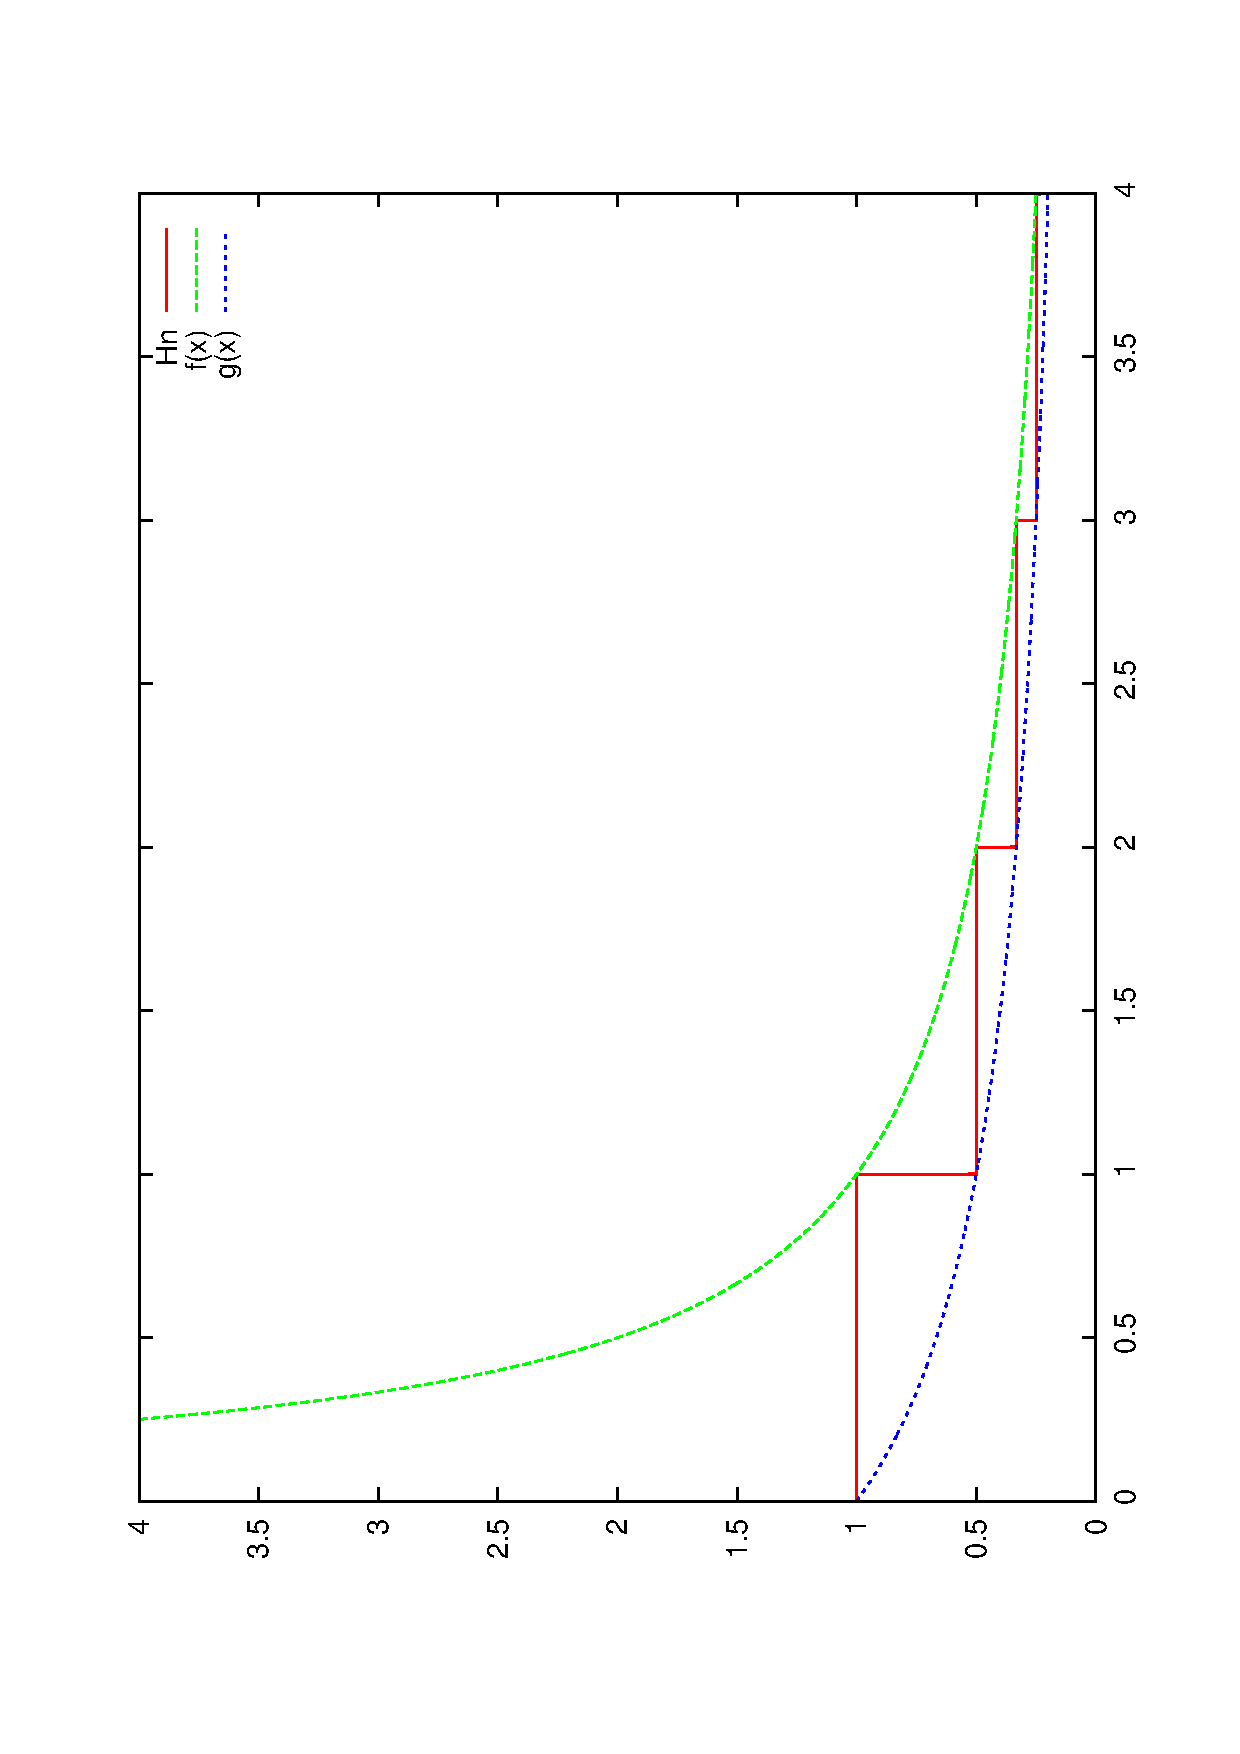
\includegraphics[width=.85\textwidth]{kap1harmonische}
  \caption{$H_n$ zeigt den Teil auf, der bei jedem Schritt der Harmonischen Reihe summiert wird. Die Harmonische Reihe kann geometrisch als die Größe der Fläche von $H_n$ interpretiert werden. $f(x)=\frac{1}{x}$ und $g(x)=\frac{1}{1+x}$ bilden eine obere und untere Schranke.}
  \label{harmonische}
\end{figure}

Die Harmonische Zahl $H_n$ kann geometrisch interpretiert werden, als die Größe der Fläche der Funktion $H_n(x) = \frac{1}{\lceil x \rceil}$, die in Abbildung \ref{harmonische} dargestellt ist. Als obere Schranken können wir $f(x) = \frac{1}{x}$, als untere $g(x) = \frac{1}{x+1}$ angeben. Also können wird $H_n$ mit Hilfe von Integralen abschätzen. Da wir $f(x) = \frac{1}{x}$ nicht von $0$ an abschätzen können, beginnen wir bei $1$ und addieren 1 für alle $ 0 \le x \le 1$ hinzu.
\begin{align*}
  H_n &\le 1 + \int_{1}^{n} \frac{1}{x} dx = 1 + \ln n - \ln 1 = 1 + \ln n \\
  H_n &\ge 1 + \int_{0}^{n} \frac{1}{x+1} dx = \ln (n+1) 
\end{align*}

Wie genau ist diese Abschätzung? Der Unterschied zwischen der oberen und unteren Schranke entspricht der Euler"=Mascheroni"=Konstante, also $\gamma \approx 0,5772156649$. Es gilt somit:
\[ H_n = \ln n + \mathcal{O}(1) \]

Jetzt haben wir alles zusammen, um die Laufzeit von Quicksort abzuschätzen.
\begin{align*}
  C(n) &\le 2(n+1) H_{n+1} \\
       &\le 2(n+1) (\ln n + \mathcal{O}(1)) \\
%       &\le (2n +2) (\ln n + 1)\\
%       &\le 2n \ln n + 2n + 2 \ln n + 2 \\
%       &\le 2n \ln n + 2(n+\ln n +1)\\
       &\le 2n \ln n + \mathcal{O}(n) \\
       &\le \frac{2n \log_2 n}{\log_2 e} + \mathcal{O}(n) \\
       &\approx 1,386 n \log n + \mathcal{O}(n)
\end{align*}
\end{Lza}

Fassen wir die Ergebnisse kurz zusammen und überlegen wir kurz, was dies für die Praxis bedeutet. Mergesort hat eine Laufzeit von $n \log n$. Quicksort hat eine Laufzeit von $1,386 n \log n + \mathcal{O}(n)$. Quicksort ist also etwa um den Faktor $1,39$ langsamer, als Mergesort.

Quicksort ist dennoch in der Realität meist effizienter als Mergesort. Mergesort muss die Daten in zwei getrennten Arrays vorhalten, Quicksort kann immer im selben Array arbeiten. Dadurch muss Quicksort weniger Daten im Speicher lesen und schreiben. Gerade bei großen Mengen kann das ausschlaggebend sein. Übersteigt der benötigte Speicher den Arbeitsspeicher eines Computers, nutzt dieser als zusätzlichen Speicher die Festplatte, was zu deutlich längeren Zugriffszeiten führt. Für bestimmte Probleme werden extra Algorithmen entwickelt, die mehr wert auf kleineren Speicherplatzverbrauch legen, als auf kurze Laufzeiten. Solche Algorithmen werden vor allem in Gebieten gebraucht, in denen Algorithmen auf großen Datenmengen rechnen, wie zum Beispiel der Meteorologie.

Abbildung \ref{groessenvergleich} veranschaulicht, die Anzahl der Vergleiche von Algorithmen bestimmter Laufzeit. Des Weiteren wird die Größe von Problemen verglichen, die ein Computer lösen kann, der $10^9$ beziehungsweise $10^{10}$ Vergleiche pro Sekunde bewältigen kann.

\begin{figure}[hbt]
  \centering
  \subfloat[Anzahl von Vergleichen für Algorithmen bestimmter Laufzeiten]{
    \begin{tabular}{>{$}r<{$}>{$}r<{$}>{$}r<{$}>{$}r<{$}}
      n & n \log n & \frac{1}{2} n^2 - \frac{1}{2} n & n! \\\hline\hline
      10 & 33 & 45 & 3{,}6 \cdot 10^{6} \\
      20 & 86 & 190 & 2{,}4 \cdot 10^{18} \\
      50 & 282 & 1225 & 3{,}0 \cdot 10^{64}\\\hline\hline
    \end{tabular}
  }
  
  \subfloat[Größe von Problemen, die eine Maschine lösen kann, welche $10^9$ Vergleiche in der Sekunde verarbeitet]{
    \begin{tabular}{l>{$}r<{$}>{$}r<{$}>{$}r<{$}}
                  & n \log n        & \frac{1}{2} n^2 - \frac{1}{2} n & n! \\\hline\hline 
      $1$ Sekunde & 4 \cdot 10^7    & 4 \cdot 10^4 & 13 \\
      $1$ Stunde  & 1 \cdot 10^{11} & 2{,}6 \cdot 10^6 & 16\\\hline\hline
    \end{tabular}
  }
  \quad
  \subfloat[Größe von lösbaren Problemen auf einer zehnmal schnelleren Maschine]{
    \begin{tabular}{l>{$}r<{$}>{$}r<{$}>{$}r<{$}}
                  & n \log n            & \frac{1}{2} n^2 - \frac{1}{2} n & n! \\\hline\hline 
      $1$ Sekunde & 3{,}5 \cdot 10^8    & 1 \cdot 10^5                    & 14 \\
      $1$ Stunde  & 9{,}1 \cdot 10^{11} & 8{,}4 \cdot 10^6                & 17 \\\hline\hline
    \end{tabular}
  }
  \caption{Übersicht über die Vergleiche bei Algorithmen bestimmter Laufzeitklasse und ihre lösbarkeit auf Maschinen verschiedener Größe.}
  \label{groessenvergleich}
\end{figure}

Man sieht in Abbildung \ref{groessenvergleich}, dass die Größe der Probleme nicht proportional mit der Geschwindigkeit des Computers wächst. Ein Computer kann alle Permutationen einer Folge untersuchen, die gerade mal ein Element mehr enthält, als es ein Computer kann, der zehnmal langsamer ist.

\section{Berechnungsmodelle (models of computing)}
Wenn wir Laufzeiten betrachten, sprechen wir bislang über Vergleiche. Wir sollten jedoch versuchen Begriffe wie Algorithmus, Speicherverbrauch und Laufzeit mathematische zu erfassen. Dazu dienen uns Berechnungsmodelle. Berechnungsmodelle sind mathematische Modelle für Rechner, also für Maschinen zum automatisierten Lösen von Problemen.

Wir wollen zwei Berechnungsmodelle betrachten. Zum einen die von Alan Turing erfundene Turingmaschine (TM), zum anderen die Registermaschine (RAM~-- random access machine). Die Definition einer Turingmaschine setzen wir als bekannt voraus.

\begin{Def}[Registermaschine (RAM~-- random access machine)]
\hspace{\parindent}
Eine Registermaschine hat einen Speicher bestehend aus einer unendlichen Anzahl an Zellen $R_0, R_1, \ldots$ Jede Zelle kann eine Zahl $\in \mathbb{Z}$ beliebiger Größe speichern.

Ein Programm ist eine endliche Folge von Befehlen. Befehle können mit einer Registeradresse $R_i$, dem Inhalt eines Registers $(R_i)$ oder einer Konstante $k \in \mathbb{N}$ arbeiten. Ein Befehlssatz könnte zum Beispiel die in Abbildung \ref{rambefehle} dargestellten Befehle umfassen.
\begin{figure}[hbt]
  \centering
  \begin{tabular}{>{\ttfamily}l@{\qquad}p{20em}}
    A := B &  wobei \texttt{A} eine Registeradresse sein muss und \texttt{B} eine Registeradressen der Form $R_i$, der Inhalt eines Registers der Form $(R_i)$ oder eine Konstanten $\in \mathbb{N}$ sein kann\\
    A := B op C & für arithmetische Operatoren, wie die Addition, Subtraktion, Multiplikation und ganzzahlige Division \\
    GOTO L & wobei \texttt{L} eine Zeile des Programms ist \\
    GGZ B, L & zur Zeile \texttt{L} des Programms springt, wenn $B > 0$ \\
    GLZ B, L & zur Zeile \texttt{L} des Programms springt, wenn $B < 0$ \\
    GZ B, L & zur Zeile \texttt{L} des Programms springt, wenn $B = 0$ \\
    HALT & Die Abarbeitung des Programms beendet.
  \end{tabular}
  \caption{Möglicher Befehlssatz einer Registermaschine}
  \label{rambefehle}
\end{figure}
\end{Def}

Die Semantik eines Befehls kann man auch formaler fassen. Den Zustand einer Registermaschine kann man durch eine Funktion $c : \mathbb{N} \to \mathbb{Z}$ beschreiben, die zu jeder Speicherzelle $R_i$ den dort gespeicherten Wert angibt. Die Semantik eines Befehls kann man dann als Abbildung eines Zustandes auf einen anderen definieren, die vollständige operationelle Semantik lässt sich also beschreiben, in dem man für alle Befehle und Zustände ihre Folgezustände angibt.

\begin{Def}[Registermaschine berechnet Funktion]
\hspace{\parindent}Die Berechnung einer Funktion durch eine Registermaschine kann man definieren als: $f : \mathbb{Z}^* \to \mathbb{Z}^*$, wobei $\mathbb{Z}^*$ die Menge aller endlichen Folgen ganzer Zahlen ist. Das bedeutet falls die Folge $a_0, a_1, \ldots, a_k$ in den Zellen $0, 1, \ldots, k$ steht, dann wird das Programm bis zum \texttt{HALT}-Befehl ausgeführt. Danach steht in den ersten $s$ Zellen $b_0, b_1, \ldots, b_s$. Das heißt, die Berechnung einer Funktion durch eine Registermaschine ist eine Funktion, die Zustände auf Zustände abbildet, wobei es eine Folge von Befehlen geben muss, die den Startzustand gegebenenfalls über Zwischenzustände in den Endzustand überführen.
\end{Def}

\subsection{Laufzeit und Speicherbedarf (Komplexitätsmaße)}
Laufzeit und Speicherbedarf eines Algorithmus dienen als Maß seiner Komplexität.

Bei Turingmaschinen sind Laufzeit und Speicherbedarf klar definiert: Ein Zeitschritt, entspricht der einmaligen Anwendung der Überführungsfunktion und damit einem Schritt des Kopfes auf dem Band der TM. Der Speicherplatz gleicht der Anzahl der benutzten Zellen auf dem Band. Formal ausgedrückt: Die Laufzeit einer TM ist definiert als $t(w) = $ Anzahl der Schritte, bis TM hält. Der Speicherbedarf einer TM ist definiert als $s(w) = $ Anzahl der benutzten Zellen des Bandes bei Eingabe $w$, bis TM hält.

Bei Registermaschinen gibt es zwei Sichtweisen, das logarithmische Kostenmaß (LKM) und das Einheitskostenmaß (EKM).

\begin{Def}[Einheitskostenmaß (EKM)]\label{defEKM}
\hspace{\parindent}Im Einheitskostenmaß kostet das Ausführen eines Befehls immer eine Zeiteinheit, unabhängig von der Komplexität des Befehls oder seinen Operanden. Für den Speicherbedarf im Einheitskostenmaß entspricht jedes Register einer Speichereinheit, unabhängig von der Größe seines Inhalts. Die Laufzeit einer Registermaschine im EKM ist also definiert als $t(x) = $ Anzahl ausgeführter Befehle bis zum ersten Erreichen des \texttt{HALT}-Befehls. Der Speicherplatzbedarf einer Registermaschine im EKM ist also definiert als $s(x) =$ in einem Schritt maximal benutzte Anzahl von Registern über alle Befehle.
\end{Def}

In der Realität wir eine Addition von zwei 1000-stelligen Zahlen mehr Laufzeit und Speicherplatz brauchen, als die Addition von zwei dreistelligen Zahlen.

\begin{Def}[Logarithmisches Kostenmaß (LKM)]\label{defLKM}
\hspace{\parindent}Das logarithmische Kostenmaß berücksichtigt die Länge der einzelnen Operanden. Die Laufzeit eines Befehls wird als die Summe der Länge der Binärdarstellung aller Werte des Befehls definiert. Ist $L(n)$ die Länge eines Operanden in Binärdarstellung, so ist die Laufzeit eines Befehls als $\sum_{i=1}^{j}L(i)$ definiert, wobei der Befehl aus den Werten $1 \ldots j$ besteht. Die Laufzeit eines Algorithmus wird wie im EKM definiert, als $t(x)=$ Summe der Laufzeiten aller ausgeführten Befehle.

Der Speicherplatzbedarf eines Zustandes im logarithmischen Kostenmaß wird als die Summe der Länge aller in Registern gespeicherter Werte in Binärdarstellung zuzüglich ihrer Adressen in Binärdarstellung definiert. Der Speicherplatzbedarf einer Registermaschine ist wieder definiert, als der in einem Schritt maximal benutzte Speicherplatz über alle Befehle. Anders ausgedrückt wird der Speicherplatzbedarf einer Registermaschine im logarithmischen Kostenmaß definiert, als der Speicherplatzbedarf des Zustands, der vom Start der Berechnung bis zum Erreichen das \texttt{HALT}-Befehls den meisten Speicherplatz verbraucht hat.
\end{Def}

\subsection{Komplexität}
Komplexität ist der Überbegriff für die unterschiedlichen Komplexitätsmaße, wie Laufzeit und Speicher. Wir unterscheiden dabei drei Fälle: die Komplexität im schlechtesten, im mittleren Fall und die erwartete Komplexität bei Zufallsalgorithmen.

Zur Berechnung des schlechtesten Falls betrachten wir das untersuchte Komplexitätsverhalten über alle Eingaben der Länge $n$ und nehmen davon das Maximum:
\begin{align*}
  T(n) &= \max_{|x|=n} t(n) \\
  S(n) &= \max_{|x|=n} s(n)
\end{align*}

Im Mittel gilt, dass $T(n)$ der Erwartungswert von $t(x)$ ist, wobei $x$ eine Eingabe der Länge $n$ ist. Zum Berechnen des Erwartungswertes brauchen wir die Wahrscheinlichkeitsverteilung auf der Menge der Länge der Eingaben. Bei der Analyse des deterministischen Quicksort-Algorithmus gehen wir davon aus, dass alle Permutationen der Eingabefolge mit gleicher Wahrscheinlichkeit auftreten.

Zufallsalgorithmen werden auch probabilistische oder randomisierte Algorithmen genannt. Sie verwenden den Zufall, um einzelne Entscheidungen zu treffen, zum Beispiel für die Auswahl eines Pivotelements. Hier hilft es nicht über alle Eingaben zu mitteln. Statt dessen muss der Erwartungswert über alle zufälligen Entscheidungen betrachtet werden.

Der deterministische Quicksort-Algorithmus hat eine gute Laufzeit im Mittel, es gibt jedoch "`schlechte"' Eingaben, die eine schlechte Laufzeit provozieren. Der randomisierte Quicksort-Algorithmus hat ein gutes Laufzeitverhalten für alle Eingaben.

%Berechnungsmodelle: gewisse mathematische Strukturen, die man Einführt um Algorithmus, Laufzeit u.ä. Begriffe zu modellieren.
%
%Das einfachste Modell ist die Turingmaschine. Laufzeit für TM: die Anzahl der Schritte, Anzahl der angewandeten Überführungsfunktionen, Speicherplatz: benutzte Zellen auf dem Band. Üblicherweise nimmt man das maximum über alle Angaben der Länge n. Man kann auch den Erwartungswert nehmen, dann spricht man von Mittel.
%
%Als weiteres Modell wurde die Registermaschine besprochen (abgekürzt RAM). Zwei Sichweisen: das Einheitskostenmaß (EKM). Egal wie groß die Operanden sind zählt man bei der Ausführung immer eine Zeiteinheit. Daher nicht ganz fair. Das logarithmischen Kostenmaß (LKM) zählt die länge der Binärdarstellungen aller beteiligten Operanden.
%\clearpage

\subsection{Vergleich dieser Berechnungsmodelle}
\begin{Satz}[Zur Laufzeit von RAM und TM]
\hspace{\parindent}Zu einer Registermaschine mit Laufzeit $T(n)$ im logarithmischen Kostenmaß gibt es eine äquivalente Einband-Turingmaschine der Laufzeit $\mathcal{O}(T(n))^5$
\end{Satz}

\begin{Satz}[Zum Speicherplatz von RAM und TM]
\hspace{\parindent}Zu einer Registermaschine mit Speicherplatz S(n) im logarithmischen Kostenmaß gibt es eine äquivalente Einband-Turingmaschine mit Speicherplatzbedarf $\mathcal{O}(S(n))$.
\end{Satz}

Insbesondere gilt, dass alle Probleme, die in polynomieller Zeit oder Platz auf einer Registermaschine mit logarithmischen Kostenmaß lösbar sind, auch in polynomieller Zeit auf einer Turingmaschine lösbar sind. Polynomiell bedeutet, dass die Laufzeit in $\mathcal{O}(n^k)$ liegt, für ein $k \in \mathbb{N}$.

\begin{Bem}[Komplexitätsklasse \textsf{P}]
\hspace{\parindent}Diese Klasse von Problemen, die in polynomieller Laufzeit lösbar sind, heißt \textsf{P}. Die Klase von Problemen, die in polynomiellem Speicherplatz lösbar sind, heißt \textsf{PSPACE}.
\end{Bem}

\section{Darstellung von Algorithmen und ihre Laufzeitanalyse}
\subsection{Pseudocode}
Algorithmen werden meist nicht als Register- oder Turingmaschinen dargestellt, stattdessen werden Konstrukte höherer Programmiersprachen genutzt, wie z.B. \texttt{if}, \texttt{for}, \texttt{while} oder Rekursion, zum Teil sogar vermischt mit umgangssprachlichen Anweisungen. Diese Art der Darstellung nennt man \textit{Pseudocode}.

Die Umsetzung in Code einer Registermaschinen sollte offensichtlich sein. Die Analyse von Algorithmen ist auch möglich, wenn sie in Pseudocode vorliegen, zumindest in Form von $\mathcal{O}$ oder $\Theta$.

\subsection{Beispiel Sortieralgorithmen}
Betrachten wir zum Beispiel die Sortieralgorithmen \ref{Bogosort} bis \ref{Alter-Mann}. Ihre Laufzeit\footnote{So nicht anders angegeben betrachten wir Laufzeit, Speicherplatz usw. immer im Einheitskostenmaß. Betrachten wir solche Werte nach dem logarithmischen Kostenmaß, weißen wir speziell darauf hin.} auf einer Registermaschine ist proportional zur Anzahl der Vergleiche. Das ist keine triviale Aussage, sondern eine Aussage, die unter Betrachtung der Algorithmen im Pseudocode gewonnen werden kann. Damit ist zum Beispiel die Laufzeit von Mergesort $\Theta(n \log{n})$ auf einer Registermaschine.

\begin{center}
\begin{tabular}{lcc}
 & Anz. Vergl. & RAM (EKM) \\\hline\hline
Minimum Auswahl & $ \frac{1}{2} n^2 $ & $2{,}5 n^2$ \\
Mergesort & \textasciitilde $n \log{n}$ & $12 n \log{n}$ \\
Randomisiertes Quicksort & \textasciitilde  $1{,}38 n\log{n}$ & $9 n \log{n}$ \\\hline\hline
\end{tabular}
\end{center}

\subsection{Rekursion}
Rekursion wird zum Beispiel von der Algorithmen-Entwurfsstrategie divide~\& conquer (Teile und herrsche) genutzt. Um ein Problem der Größe $n$ zu lösen, wird es in kleinere Teilprobleme zerlegt. Diese löst man rekursiv und kombiniert ihre Lösungen zu einer Lösung des Gesamtproblems.

Liefert die Laufzeitanalyse eines Algorithmus eine Rekursionsgleichung, so muss diese aufgelöst werden (vergleiche z.B. die Laufzeitanalyse \ref{QuicksortLza} von Quicksort auf S. \pageref{QuicksortLza}). Die Nutzung von Rekursion in Algorithmen beinhaltet die Gefahr exponentielle Laufzeit zu bekommen (siehe Übung).

Neben der Laufzeit spielt auch der Platzbedarf gerade bei rekursiven Algorithmen eine große Rolle. Während der Laufzeit wird ein Stack aufgebaut, der für alle rekursiven Aufrufe einen activation record, einen Datensatz mit allen Laufzeitinformationen, enthält. Unter der Annahme, dass die Datensätze im Laufzeitstack konstante Größe haben, ist der Speicherplatzbedarf für diesen Stack ist so hoch, wie die Tiefe der Rekursion sein kann.

\begin{Bsp}[Fakultät]
\hspace{\parindent}
Die Fakultät lässt sich rekursiv berechnen:
\begin{align*}
fak(0) &= 1 \\
fak(n) &= fak(n-1) \cdot n
\end{align*}

Dieses Vorgehen hat einen Speicherplatzbedarf von $\Theta (n)$. Die Fakultät lässt sich aber auch durch eine einfache Schleife berechnen, ganz ohne Rekursion und ohne Laufzeitstack.
\end{Bsp}

\subsection{Typische Funktionen}

Betrachten wir einige bei der Analyse von Algorithmen typischerweise auftretende Funktionen, sortiert nach ihrem Wachstum:
\begin{center}
\begin{tabular}{cll}
$\log{\log{n}}$ & \multirow{2}*{$\left.\vphantom{\begin{array}{l}\\\end{array}}\right\rbrace$logarithmisch}\\
$\log{n}$\\
$\sqrt{n}$\\
$n$ & linear & \multirow{4}*{$\left.\vphantom{\begin{array}{l}\\ \\ \\ \end{array}}\right\rbrace$polynomiell}\\
$n \log{n}$\\
$n^2$ & quadratisch\\
$n^3$\\
$\vdots$\\
	$2^n$ & \multirow{3}*{$\left.\vphantom{\begin{array}{l}\\\\\end{array}}\right\rbrace$exponentiell}\\
$n!$\\
$2^{n^2}$\\
$2^{2^n}$ & doppelt exponentiell\\
\end{tabular}
\end{center}

Da $\lim\limits_{n \rightarrow \infty}{\frac{\log{n}}{n^\alpha}} = 0$ wissen wir, dass $\log{n} = o(n^{\alpha})$. $\log{n}$ wächst also schwächer als jedes $n^\alpha, \alpha > 0$, daher auch als $\sqrt{n} = n^{\frac{1}{2}}$.

